\section{ SR0013CN19 }


\subsection{Meta}

    \textbf{Title:}
    Operating room planning and surgical case scheduling: a review of literature

    \begin{table}[H]
        \centering
        \begin{tabular}{|c|c|c|c|c|c|c|c|c|}
            \hline
                \textbf{Rank} & \textbf{Grasp} & \textbf{Grade} & \textbf{Type} & \textbf{Outcome} & \textbf{Domain} & \textbf{COV19} & \textbf{CoI} & \textbf{DB} \\
            \hline
                5 & 95\% & B & A & P & S & No & Yes & No \\
            \hline
        \end{tabular}
        \caption{Reference's metadata}
        \label{tab:SR0013CN19}
    \end{table}

\subsection{Summary}
    Shuwan Zhu et al. \cite{x203} provided a literature review with classification considering operating room planning and scheduling. From the construction point of view, the paper is very similar to \cite{x029}. For instance, both studies concentrate on the scheduling problems, not the solutions, but with some noteworthy differences. First, the study demonstrates quantitative literature analysis, absent from \cite{x029}. Second, the paper's structure is looser, and finally, the terms and definitions are more up-to-date. On the other hand, the authors of \cite{x029} proposed more concrete and fundamental explanations for terms in healthcare planning and scheduling. Ultimately, this paper represents a valuable asset for newcomers in the field regarding terminology and general trends.

\subsection{Notes}
    \begin{itemize}
        \item PubMed, Web and Science, IEEE, Springer, and Inspec;
        \item Terms definitions;
    \end{itemize}


\subsection{Reading}
    \textbf{Abstract:}
    It is a comprehantice review of studies in the operating room planning and surgery case scheduling. The interested aspects of the review are: decision levels, scheduling strategy, patient characteristics, problem definition, uncertainty, and solution approaches. The quantitative analysis of the existing publications shows that the most interested planners are build with math models and heuristics.
    
    \textbf{Objectives:}
    ??
    
    \textbf{Page 1:}
    Operating theatres are a focal point in improving medical care efficiency for most hospitals.
    
    \textbf{Page 2:}
    The number of literature reviews show that the operating room planning is a field of high scientific interest. The authors overviewd 315 studies, where more then half were published after 2010.
    \begin{figure}[H]
        \centering
        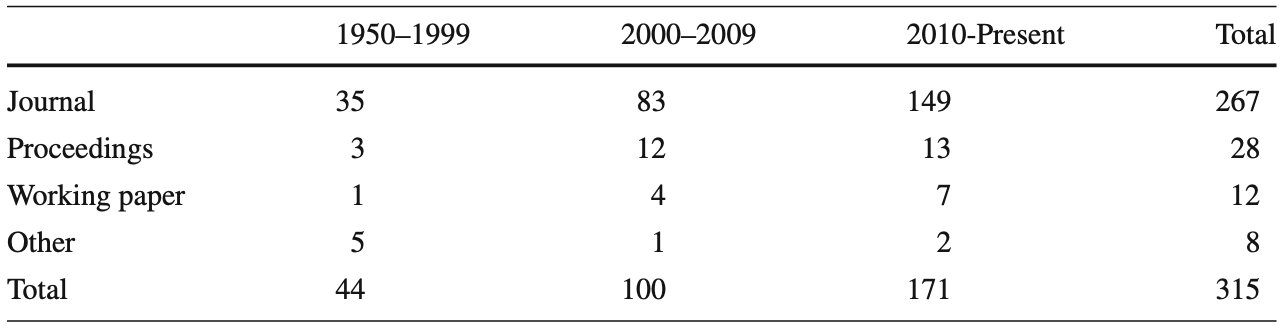
\includegraphics[width=1\textwidth]{figures/SR0013CN19/fig1.png}
        \caption{Distribution of reviewved works by type and year of publication \cite{x203}.}
        \label{fig1:SR0013CN19}
    \end{figure}
    
    \textbf{Page 3:}
    The literature review convers six aspects of the operational room planning: desicion levels, scheduling strategies, patient characteristics, problem features, math models, solutions and methods. The decision classification includes strategic, tactical, and operational levels of decision-macking. To strategic level problem can be related: capacity planning problem, capacity allocation problem, and case-mix problem.
    \begin{figure}[H]
        \centering
        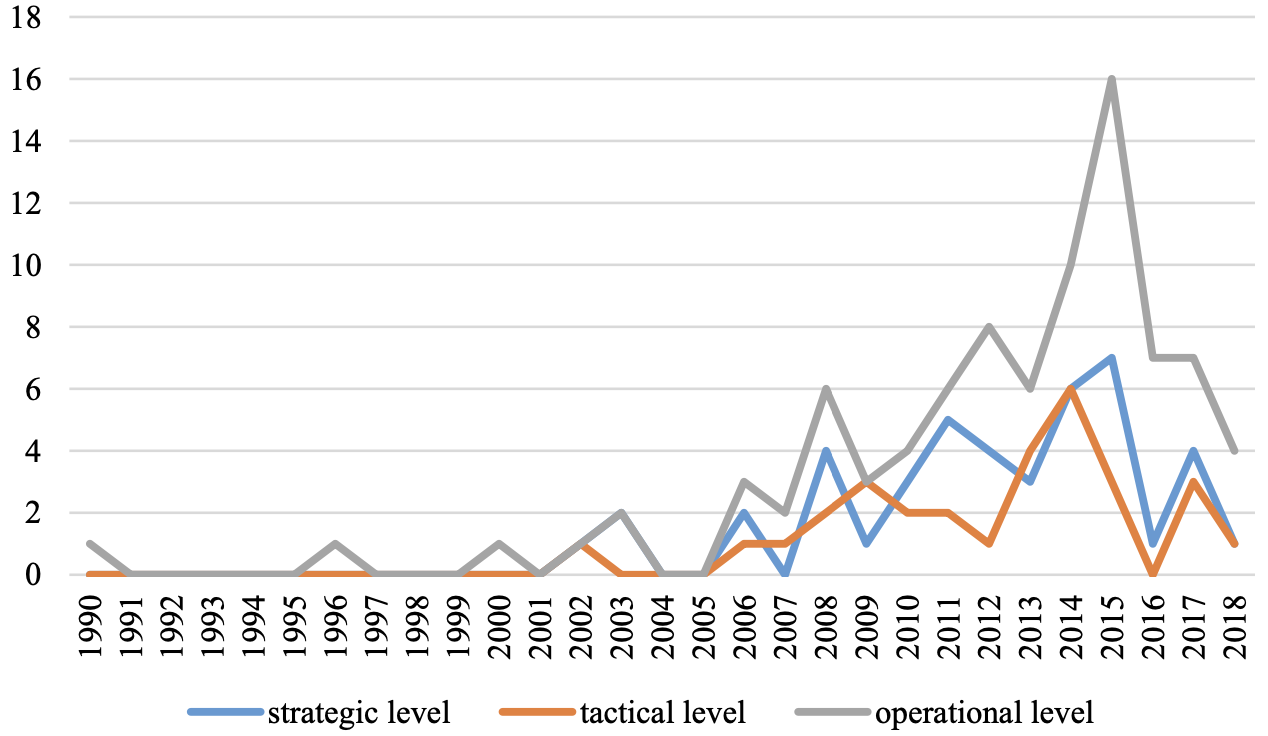
\includegraphics[width=1\textwidth]{figures/SR0013CN19/fig2.png}
        \caption{Publication trends classified by desicion levels in \cite{x203}.}
        \label{fig2:SR0013CN19}
    \end{figure}

    \textbf{Page 4:}
    Capacity planning = resouces + demand-capacity balance.
    
    \textbf{Page 5:}
    Capacity allocation = long-term horizon + operating room + specialities.
    Case-mix problem (CMP) = long-term horizon + resource  + time blocks.
    
    \textbf{Page 6:}
    Tactical level = mediom-size horizon (month, quartal) + cyclic schedule + resouce allocation + specific times / time blocks / flexible time blocks. (reflection: the tactical level gets so far more attention then the strategic level description).
    
    \textbf{Page 7:}
    Operating level (Surgeon Scheduling Problem (SSP), Patient Scheduling Problem) = advance scheduling and allocation. Advance scheduling (intervention assignment, surgery case assignment) = surgery case + date of operation + operation room. 
    
    \textbf{Page 8:}
    Allocation scheduling (intervention schediling, surgical case scheduling) = waiting list + day plan + possible pre-assignments.   
    
    \textbf{Page 9:}
    Some studies develop an integration of advance scheduling and allocation scheduling together, and even consider downstream capacities. (reflaction: it is the sence of practical model, isn't it?). Scheduling strategies involve: block strategy, open strategy, and modified block strategies.

    \textbf{Page 10:}
    Block scheduling strategies = fixed time and/or fixed patient group and/or fixed resouces which are considered in blocks.

    \textbf{Page 11:}
    Open scheduling strategy = open time slots + FIFO (FCFS). The authors of this review criticise the open scheduling strategy due to low utilisation of the medical resources and often unstructured workflow for surgeons.
    
    \textbf{Page 12:}
    Modified block scheduling strategy = combination of block and open scheduling strategies. A comment from the authors - it is harder to manage, and the there are ongoing research in the direction of modified block scheduling strategy. There are two segments of patients: elective or non-elective patients, and inpatients or outpatients. 

    \textbf{Page 13:}
    Inpatients and outpatients: list of related publications and no new information.
    
    \textbf{Page 14:}
    Elective and non-elective patients: elective patients can be conventional (= inpatiets) or ambulatory (= outpatients). Non-elective patients' subclasses are emergent and urgent (reflection: sometimes could be semi-urgent cases). Most of the research focuses on the elective patients, the patients which are predominant in hospitals. Another important factor, uncertainty considered for more practical scheduling models.
    
    \textbf{Page 15:}
    Uncertainty is a significant aspect for the medical resource scheduling. Most of the studies ignore it, and some try to conquer unsertanties using methods with stohastic nature.
    
    \textbf{Page 16:}
    \begin{figure}[H]
        \centering
        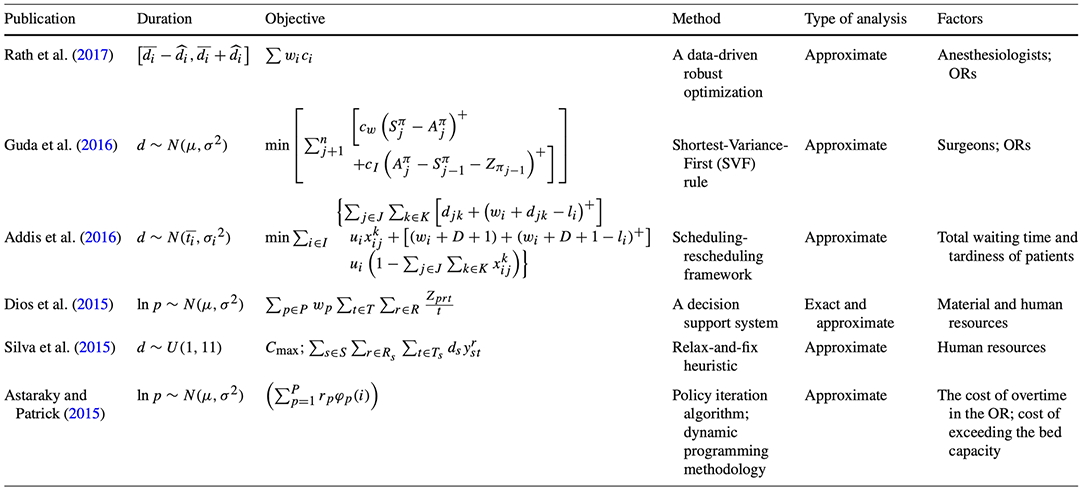
\includegraphics[width=1\textwidth]{figures/SR0013CN19/fig3.png}
        \caption{Some objectives from literature by \cite{x203}, part I.}
        \label{fig3:SR0013CN19}
    \end{figure}
    
    \textbf{Page 17:}
    \begin{figure}[H]
        \centering
        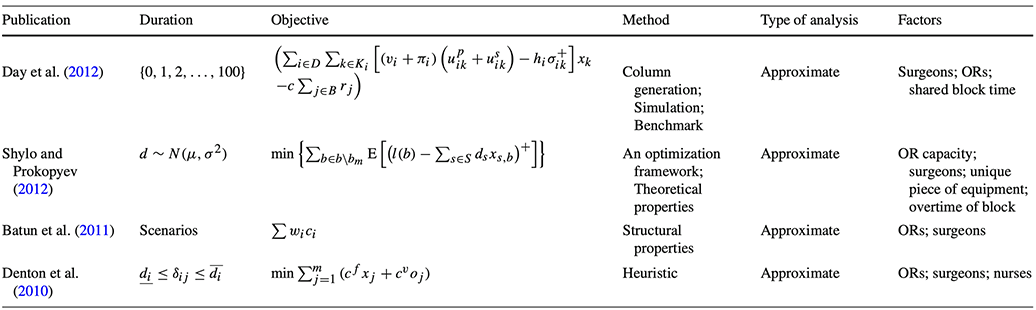
\includegraphics[width=1\textwidth]{figures/SR0013CN19/fig4.png}
        \caption{Some objectives from literature by \cite{x203}, part II.}
        \label{fig4:SR0013CN19}
    \end{figure}
    
    \textbf{Page 18:}
    \begin{figure}[H]
        \centering
        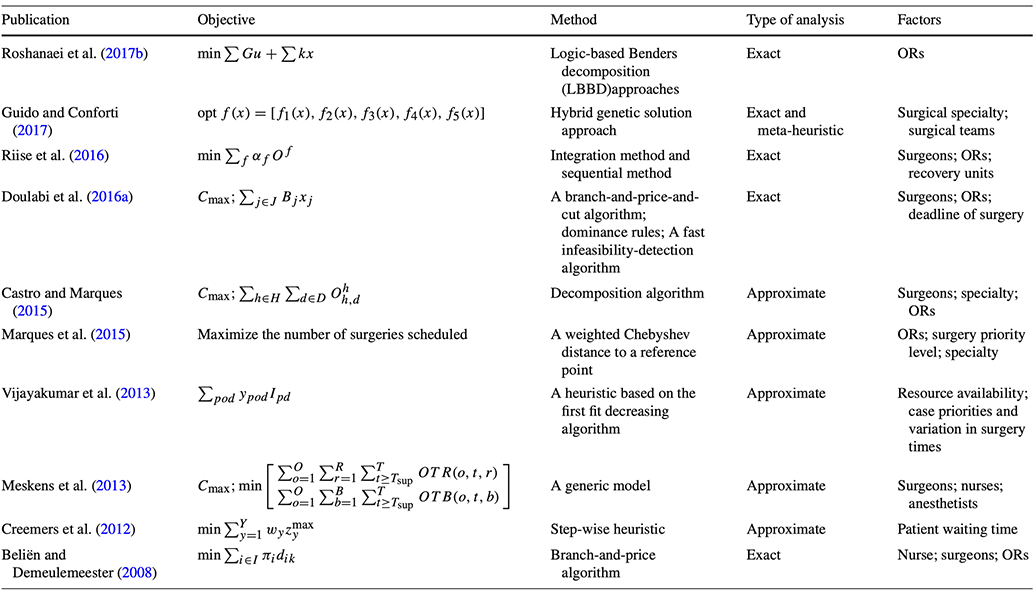
\includegraphics[width=1\textwidth]{figures/SR0013CN19/fig5.png}
        \caption{Some objectives from literature by \cite{x203}, part III.}
        \label{fig5:SR0013CN19}
    \end{figure}

    \textbf{Page 19:}
    This page starts with list of papers categorised by type of uncertainty. Then the duration uncertainty is explained as "deviations between the actual and planned durations of relecant activities during the surgical process".

    \textbf{Page 20:}
    The modeling of uncertainty is split into to dirations: using Monte Carlo simulation, or using random probability distribution (lognormal, gamma, and normal).
    \begin{figure}[H]
        \centering
        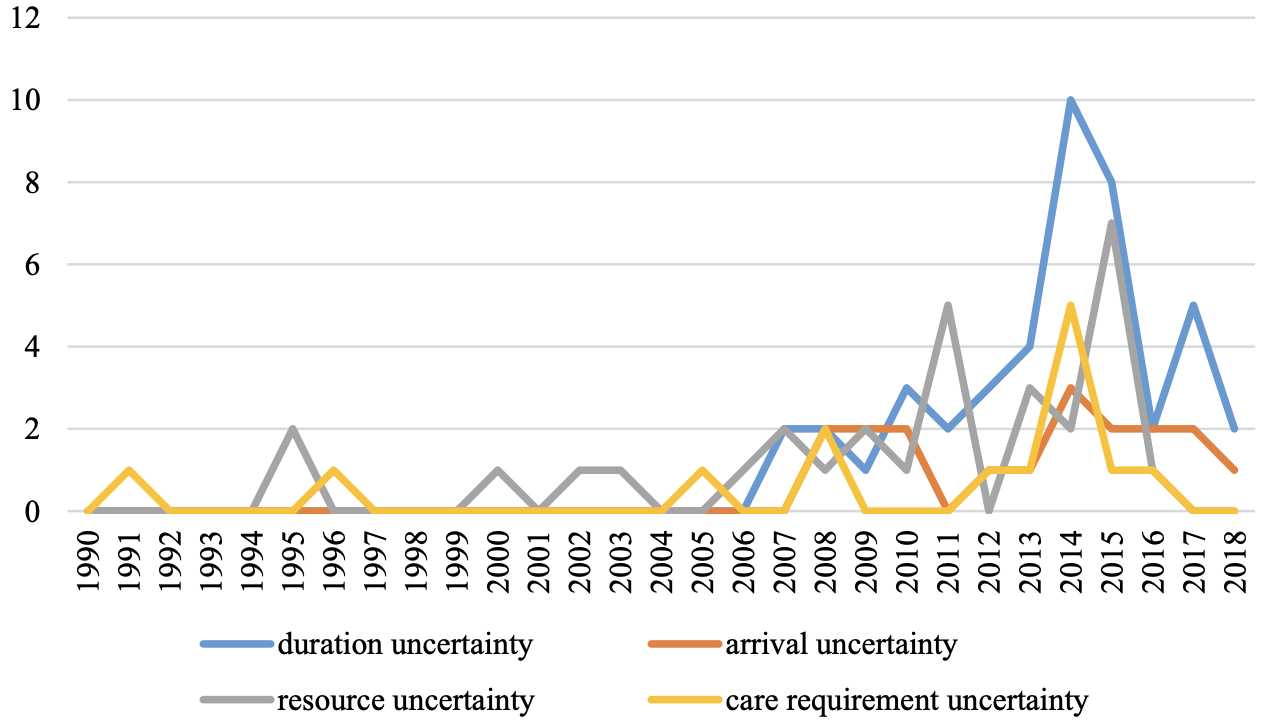
\includegraphics[width=1\textwidth]{figures/SR0013CN19/fig6.png}
        \caption{Trends in publications with uncertainties over the years from \cite{x203}}
        \label{fig6:SR0013CN19}
    \end{figure}

    \textbf{Page 21:}
    \underline{Arrival uncertainty}: not much new, sturied with simulation techniques to find a better solution to reduce arrival uncertainty factor. \underline{Resource uncertainty}: unexpected equipment breack down, supply shortage, etc. \underline{Care requirement uncertainty}: the other objectives which can pop-up on the way (reflaction: not clear explanation).
    
    \textbf{Page 22 (Objective functions):}
    \underline{Certain requirement}: infection cleaning and the discussion ergarding this in the reviewed publications. In addition, there could be patient specific requirements. 
    
    \textbf{Page 23 (Objective functions):}
    ... some authors design models which take into account three surgery priority levels and also human resources such as surgeons and nurses. Next is a description of multi-stage scheduling approache implemented in some of the studies. First - assign resource to operation room and caregivers; second - define the start time for the surgery. 
    
    \textbf{Page 24 (Math models):}
    Surgery planning and scheduling problem was translated into bin-packing, flow-shop, stochastic, and multi-critaria model. \underline{Bin-packing model}: ORs = bins, surgery cases = items to be packed. There are on- and off-line bin-packing models.
    
    \textbf{Page 25 (Math models):}
    \underline{Flow-shop model}: described as NP-hard problem and then the relevant studies were presented. \underline{Stochastic model}: adds uncertainties into idealised models. \underline{Multi-criteria model}: fewver works explisitly use multi-criteria models.
   
    \textbf{Page 26 (Solutions and methods):}
    \underline{Exact algorithm}: always optimal, small-scale problem, examples: column generation, dynamic programming, branch and cut, branch and bound, and branch-and-price.
    
    \textbf{Pages 27-29 (Solutions and methods):}
    These pages outline and show examples of the exact algorithm implementation in the reviewed papers. (reflaction: the algorithms themselves are not explained).
    
    \textbf{Page 30 (Solutions and methods):}
    \underline{Heuristics} are divided into six categories: based on exact methods, constructive, improvement, meta-heuristics, linear programming (LP) based, and dispatching-rule based. 

    \textbf{Pages 31-34 (Solutions and methods):}
    Tables with studies classified to different heuristic methods.
    
    \textbf{Pages 35-36 (Solutions and methods):}
    List of the literature with solutions.
    
    \textbf{Page 37 (Solutions and methods):}
    \underline{Simulations}: provide evaluation of the solution models for broader spectrum of cases. In sume publications, simulation approaches are used as primary solution model. The authors separate Monte Carlo simulation, Dicrete-event simulation ad others.
    
    \textbf{Page 38 (Solutions and methods):}
    \underline{Markov decision process (MDP)}: is practical for veriaty of optimisational approaches that focuse on on dynamic programming and reinforcement learning.
    
    \textbf{Pages 38-39 (Conclusions):}
    The operating room scheduling is a complex task. The authors conducted a literature review and classified the studies in multiple sections and subsections. Majority of the research dedicated to short-term horizons. The unsertainties are often ingnored which is not practical considering the unpredicitble nature of the operating rooms scheduling problem.
